\section{Введение}
\subsection{Актуальность работы}

Кровь -- соединительная ткань внутри организма, она состоит из форменных клеток (эритроцитов, лейкоцитов, тромбоцитов), а так же из
водного раствора белков и свёртывающих веществ -- плазмы. Кровь под воздействием периодических сокращений сердечной мышцы 
движется по замкнутой системе сосудов, циркулируя от сердца и обратно. С точки зрения гидродинамики кровоток представляет 
из себя пульсирующее с низкой частотой течение мелкодисперсной суспензии в 
замкнутой системе каналов кругового сечения с эластичными стенками, осложнённое локальными эффектами ламинарно-турбулентного перехода.

Кровь, двигаясь по сосудам, испытывает сопротивление движению со стороны сосудов и из-за своей вязкости. Поэтому сердце вбрасывает 
кровь в сосуды под большим давлением. В аорте давление колеблется в диапазоне от 120~мм рт.ст. при систоле до 80~мм рт.ст. при диастоле. 
По мере движения крови давление в сосудистом русле падает. 
Скорость течения крови так же зависит от диаметра сосуда, удалённости сосуда от сердца, а также фазы сердечного цикла. 
Максимальных значений скорость достигает в аорте (до \texttilde$1$~м/с), а минимальных -- в капиллярах (около нуля).

Сложность разветвления кровеносных сосудов и вариации их размеров создают значительные трудности при решении задачи о течении крови. 
Математическое моделирование помогает  
аппроксимации и пониманию сложностей кровотока. Эти модели позволяют описывать и строить физические процессы, происходящие 
в биологических областях, что может быть полезно при выявлении, прогрессировании и лечении  различных сердечно-сосудистых заболеваний , 
а так же в проектировании и оптимизации медицинских устройств.

Описывать кровь можно различными способами. Например, детально: кровь состоит из взвешенных в плазме 
(которую чаще рассматривают, как ньютоновскую жидкость) клеток крови, которые действуют друг на друга с некоторыми силами. 
Описание такого типа методов можно подробнее изучить в ~\cite{Fedosov:2010,Fedosov:2008,Mehboudi:2001}. 
В некоторых моделях ~\cite{bessonov:2014,hosseini:2009} пренебрегают относительно мелкими и редкими -- тромбоцитами
(2--4~мкм в количестве 150--300 миллионов на 1~см$^3$) и лейкоцитами(4--20~мкм в количестве 4.5 -- 11 миллионов на 1~см$^3$), 
а строят двумерные сетки, состоящие только лишь из эритроцитов (7 -- 8~мкм в количестве 3.8 до 5.6 миллиардов клеток на 1~см$^3$).
Но при таких подходах можно столкнуться с некоторыми проблемами: такую модель будет сложно сравнивать как
с другими моделями, так и с эксперементальными показателями, так же она очень плохо реагирует на любые изменения в исходных данных. 
Соответсвенно, возникает необходимость прибегнуть к дальнейшему осреднению.

Можно не описывать индивидуальные частицы взвешенные в плазме, а обобщить их до вязкой неньютоновской жидкости с определёнными 
характеристиками, тогда любые изменения можно будет отразить в параметрах жидкости. Такой подход называют трехмерным моделированием.
Существует множество трёхмерных моделей, например, основанные на зависимости вязкости от гематокрита ~\cite{walburn:1976},
модель Максвелла \cite{thurston:1972},  модель Кассона ~\cite{moller:2006}.
Однако эти модели всё-таки требуют значительных вычислительных ресурсов, а следовательно, и дальнейших упрощений. 

Для вывода граничных условий в трёхмерных моделях иногда используют одномерное моделирование, которое может быть 
и вполне самостоятельным подходом к моделированию течения крови.
В одномерных моделях пространственные характеристики осредняются по поперечному сечению, а трёхмерная дифференциальная
задача сводится к одномерной. Такой подход к моделированию требует меньших вычислительных ресурсов, но при этом почти не уступает в 
точности другим моделям. О сравнении одномерных и многомерных моделей можно прочитать в ~\cite{FORMAGGIA:2001}.

Вычислительной областью модели является сосудистая одномерная сеть или же её части. Сеть создаётся на основе общих анатомических данных,
например, справочник анатомических карт ~\cite{bunicheva:2013}, анатомические 3D модели или данные конкретного человека или животного. 
Задаётся так же и физические характеристики крови, такие как плотность: обычно её оценивают в 1052 -- 1060~кг/м\textsuperscript{3},
вязкость (4.3 -- 4.9~мПа$\cdot$). 



Для построения модели нужно выбрать подходящий метод.

Метод конечных разностей предполагает дискретизацию области на сетку точек и последующую аппроксимацию производных в управляющих
уравнениях с помощью конечных разностей. Этот метод часто используется в сочетании со схемой интегрирования по времени для решения 
полученной системы обыкновенных дифференциальных уравнений.

Метод конечных элементов~\cite{TAYLOR1998} -- популярная численная схема. 
Он особенно хорошо подходит для моделирования сложных геометрий, таких как запутанная сеть артерий в человеческом теле. 
Однако он может быть вычислительно дорогим, особенно для больших и сильно разветвленных сетей. 

Метод быстрого преобразования Фурье~\cite{Sazonov:2019} -- 
это подход, использующий быстрое преобразование Фурье для решения одномерных уравнений кровотока. 
Этот метод конкурирует с традиционными пространственно-временными численными схемами как по устойчивости, так и по скорости. 
Он может точно и эффективно обрабатывать сложные геометрические формы и высокоамплитудные волны. 
Однако он требует дальнейшего развития для учета вязкоупругих эффектов и потери массы крови из-за мелких ветвей. 

Метод прерывистого Галеркина~\cite{yao:2017} -- это еще одна численная схема, она сочетает в себе преимущества методов конечной разности и конечных элементов, 
обеспечивая баланс между точностью и вычислительными затратами. Однако он может быть более сложным в реализации и может
потребовать дополнительных вычислительных ресурсов для сопоставления расчетной и физической областей.

Метод конечных объемов с локальным временным шагом высокого порядка~\cite{mueller:2015} предполагает решение управляющих уравнений 
с помощью метода конечных объемов высокого порядка и схемы локального шага по времени. 
Этот метод может быть особенно полезен для моделирования течения в сложных геометрических системах.

{\bf Постановка задачи}

Описывающие течение крови модели выводятся путём усреднения уравнений Новье-Стокса~\cite{Formaggia:2009}. 

По второму закону Ньютона движение среды определяется действием массовых и поверхностных сил. 
Законы сохранения массы и импульса для сплошной среды могут быть
записаны в переменных $(A, u, p)$: 
\begin{align}
    \label{eq:mass-balance}
    \varphi=&\frac{\partial A}{\partial t}+\frac{\partial Au}{\partial x},\\
    \label{eq:momentum-balance}
    \psi=&\frac{\partial u}{\partial t}+ \frac{\partial u^2/2+p/\rho}{\partial x}
\end{align}
Здесь $t$ -- время, $x$ -- координата вдоль сосуда, $A(t, x)$ -- площадь поперечного сечения сосуда, 
$u(t, x)$ и $p$ -- усредненная по сечению линейная скорость и трансмуральное давление крови. 

В системе три неизвестных: $(A, u, p)$, поэтому в каждой конечной точке сосуда требуется одно дополнительное условие совместимости.
Например, сохранение массы:
\begin{equation}
    \label{eq:conserv-mass}
    \sum_{k=k_1,k_2,...,k_N} \varepsilon_k A_k(t,x_k)u_k(t,x_k)=0,
\end{equation}
где {$k_1,...,k_N$} -- индексы сосудов, $\varepsilon_k=1, x_k=0$ -- для входящих сосудов,
$\varepsilon_k=1, x_k=L_k$ -- для выходящих сосудов.
Также используется $N$ интегральных условий сохранения Бернулли выражающих непрерывность полного давления $P^l$:
\begin{equation}
    \label{eq:bernulli}
    \frac{\rho u^2_k}{2}+{p_k(A_k)}=P^l.
\end{equation}
Иногда для моделирования сопротивления потоку в местах стыка используют условия перепада давлений
с учётом сопротивления
\begin{equation}
    \label{eq:p-pressure}
    p_k\left(A_k\left(t,x_k\right)\right)-p^l(t)=\varepsilon_k R^l_k A_k(t,x_k)u_k(t,x_k),
\end{equation}
которое выражается через коэффициент $R^l_k$. Здесь $p^l$ -- давление в точке бифуркации \cite{bessonov:2014}.

Многие авторы~\cite{alastruey:2008} выполняют сопряжение во временной области 1D моделей кровотока с электрическими цепями
(единичными параметрами) 0D моделей. 0D модели обеспечивают корректные граничные условия для глобальных моделей кровотока.

Но общим способом замыкания системы является явное представление алгебраической зависимости
между давлением в сосуде и его площадью. Прямой подход к получению отношения $p(A)$ включает в себя точное одновременное измерение
давления и площади в разные моменты времени. Но такой метод не всегда удобен в реальности.
Качественный анализ физических экспериментов подтверждает, что функция $p(A)$ должна быть монотонной S-подобной кривой. 
Такая кривая удовлетворительно описывает состояния как круглого, так и эллиптического сечения. 


\begin{figure}[h]
    \centering
    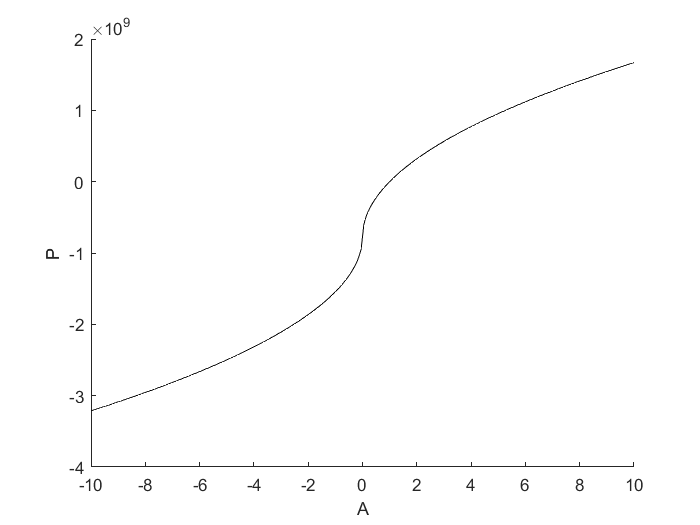
\includegraphics[width=0.6\linewidth]{PA.png}
    \caption{График зависимости давления от поперечного сечения внутри сосуда.}
    \label{ych}
\end{figure}

